\documentclass[11pt,a4paper]{article}
\usepackage[margin=24mm,headheight=15pt]{geometry}
\usepackage[T1]{fontenc}
\usepackage{lmodern,microtype,graphicx,amsmath,booktabs,longtable,tabularx,array,enumitem,xcolor,fancyhdr,tikz}
\usetikzlibrary{arrows.meta,positioning}
\usepackage[colorlinks=true,linkcolor=teal!60!black,urlcolor=teal!60!black]{hyperref}
\usepackage{listings}
\definecolor{ink}{HTML}{123047}
\definecolor{accent}{HTML}{007F82}
\definecolor{pale}{HTML}{EDF5F6}
\hypersetup{pdftitle={TraceMeet: Traceable Meeting Documentation},pdfauthor={Aditya Om Sah}}
\pagestyle{fancy}\fancyhf{}\fancyhead[L]{\small\textcolor{ink}{TraceMeet | Technical Report}}\fancyhead[R]{}\fancyfoot[C]{\thepage}
\setlength{\emergencystretch}{2em}\setlength{\parindent}{0pt}\setlength{\parskip}{6pt}
\setlist{nosep,leftmargin=*}
\setlist[description]{style=unboxed,leftmargin=0pt}
\setcounter{tocdepth}{1}
\lstset{basicstyle=\ttfamily\footnotesize,breaklines=true,frame=single,rulecolor=\color{accent},backgroundcolor=\color{pale},columns=fullflexible,keepspaces=true}
\newcommand{\code}[1]{\nolinkurl{#1}}
\newcommand{\src}[1]{\par{\footnotesize\raggedright\textcolor{accent}{Implementation:} #1\par}}
\newcolumntype{Y}{>{\raggedright\arraybackslash}X}
\begin{document}
\begin{titlepage}
\centering
\vspace*{22mm}
{\large\textcolor{accent}{INTER IIT BOOTCAMP PROJECT}}\par
\vspace{30mm}
{\fontsize{42}{48}\selectfont\bfseries\textcolor{ink}{TraceMeet}}\par
\vspace{9mm}
{\Large Every meeting. A record you can trace.}\par
\vspace{12mm}
{\color{accent}\rule{0.48\textwidth}{0.8pt}}
\vfill
{\large\textbf{Technical Design and Engineering Report}}\par
\vspace{7mm}
{\Large Aditya Om Sah}\par
\vspace{3mm}
{\large Indian Institute of Technology Guwahati}\par
\vspace{7mm}
{\small\url{https://github.com/adityaomsah/TraceMeet}}\par
\vspace{12mm}
\end{titlepage}

\section*{Abstract}
Turning meeting speech into useful documentation requires more than fluent transcription and summarization. Recognition errors can alter technical terms, refinement can change commitments, and summarization can misrepresent a proposal as an agreed action. TraceMeet addresses these risks through an end-to-end workflow that makes intermediate wording and supporting evidence inspectable.

The system separates three model roles: local faster-whisper transcribes English recordings; Gemini proposes domain-aware transcript corrections; and Groq-hosted GPT-OSS generates structured minutes, decisions, tasks and open questions. Python preserves segment identity and timestamps, computes exact correction spans, withholds proposals that trigger sensitive-change heuristics, and checks quoted evidence against the transcript. The interface retains raw, proposed and applied wording and links citations to recording playback.

For recordings that exceed the configured request budget, documentation proceeds through provisional extraction, meeting-wide grouping, source-grounded reconciliation and accounted finalization. Explicit candidate dispositions and topic accounting prevent silent loss of already-extracted items during consolidation. Input- and output-aware planning, bounded repair attempts and validated checkpoints support recovery without repeating matching completed work. Readable views and downloadable formats are generated from one citation-checked record.

Development runs demonstrate the short-recording workflow and staged processing of a 463-segment recording. These observations establish functional feasibility, not meeting-understanding accuracy. Citation matching verifies textual presence rather than semantic support; the summary remains uncited, and independent accuracy evaluation is pending. TraceMeet's contribution is an inspectable orchestration of existing models with explicit provenance, recovery and review boundaries.

\newpage
\tableofcontents
\newpage

\section{Problem definition and system objectives}
Meeting documentation can fail in several distinct ways: speech recognition can mishear terminology, refinement can change a name or commitment, and summarization can turn a suggestion into an assignment. A fluent final document conceals these failures unless intermediate representations remain visible. TraceMeet is designed to retain those representations and connect statements to recording segments.

The required workflow is upload, transcription, refinement and meeting documentation in that order. The interface must expose raw and refined transcripts separately, report unusable input clearly, and generate downloadable results for a new recording. Outputs cannot be prewritten examples. Tasks should contain an owner or deadline only when supported by the recording, and tentative proposals should not be presented as confirmed decisions.

These requirements lead to five design objectives:
\begin{enumerate}
\item Preserve stable identity between raw, proposed and applied transcript segments.
\item Place structural validation in Python rather than asking a language model to self-certify it.
\item Make uncertainty and withheld edits inspectable in the interface.
\item Retain successful stages when later model calls fail.
\item Generate readable and machine-readable exports from one checked record.
\end{enumerate}
The intended deployment is a local, single-user Streamlit application. It is not a production multi-tenant meeting service and does not implement participant diarization, enterprise access control or encrypted run storage.

\subsection{Engineering contributions}
TraceMeet's contribution is the integration of existing models with explicit, inspectable contracts. No new model architecture or model training is claimed. The distinguishing engineering work is concentrated at the handoffs where a fluent model response can otherwise become an untraceable output.
\begin{enumerate}
\item \textbf{Three-way transcript provenance:} preserve raw wording, the model proposal and the guarded wording actually used downstream.
\item \textbf{Accounted long-meeting reduction:} record the disposition of existing candidates and topics instead of silently accepting a shorter final result.
\item \textbf{Recoverable stage execution:} reuse compatible saved artifacts while invalidating stale downstream results.
\item \textbf{Inspectable delivery:} expose source playback and render the interface and downloadable formats from the same citation-checked record.
\end{enumerate}
These properties are implemented controls, not claims that no other system offers similar features. Their value must ultimately be assessed through correctness, usability and failure-recovery evidence.

\subsection{Requirements mapped to implementation}
\begin{tabularx}{\textwidth}{@{}p{0.25\textwidth}YY@{}}\toprule
Requirement & Implementation & Verification boundary\\\midrule
English recording to raw text & Media validation and local Whisper transcription & New-recording UI smoke tests reported; accent/noise accuracy not yet benchmarked.\\
Domain-aware refinement & Glossary-conditioned Gemini proposals with identity checks and sensitive-edit guards & Candidate edits remain inspectable; meaning preservation is heuristic.\\
Separate documentation model & Groq short path or map/group/reconcile/finalize workflow & Structured output and citations checked; interpretation still needs evaluation.\\
Retain both transcripts & Raw and guarded refined artifacts, with separate candidate wording & Shared IDs and timestamps support comparison and playback.\\
One interactive workflow & Streamlit processing, stage status and saved-run resume & Short recordings completed; clean-clone verification remains pending.\\
Downloadable outputs & JSON, Markdown, task CSV and ZIP from one checked record & Export consistency tests and manual ZIP inspection reported.\\\bottomrule
\end{tabularx}

\section{Architecture and model-role selection}
\subsection{Three separate processing roles}
\begin{tabularx}{\textwidth}{@{}lYY@{}}\toprule
Role & Configured implementation & Reason for this choice\\\midrule
Speech recognition & faster-whisper \code{small.en}, CPU, \code{int8} & A working local baseline that does not require a GPU or another speech API key.\\
Refinement & Gemini \code{gemini-3.5-flash-lite}, temperature 1.0 & Retains the working terminology-refinement stage while the documentation provider changes.\\
Documentation & Groq \code{openai/gpt-oss-120b}, temperature 0.0 & A separately tested structured-output candidate after repeated Gemini documentation failures.\\\bottomrule
\end{tabularx}

These are the literal configured identifiers in the implementation. Their inclusion records the implemented profile, not a claim about future model availability. An API access probe remains necessary on another account. The two language stages are distinct processing stages and use distinct configured models; the long documentation path uses multiple calls to the same documentation model, not additional independent model roles.

\subsection{Execution flow}
\begin{center}
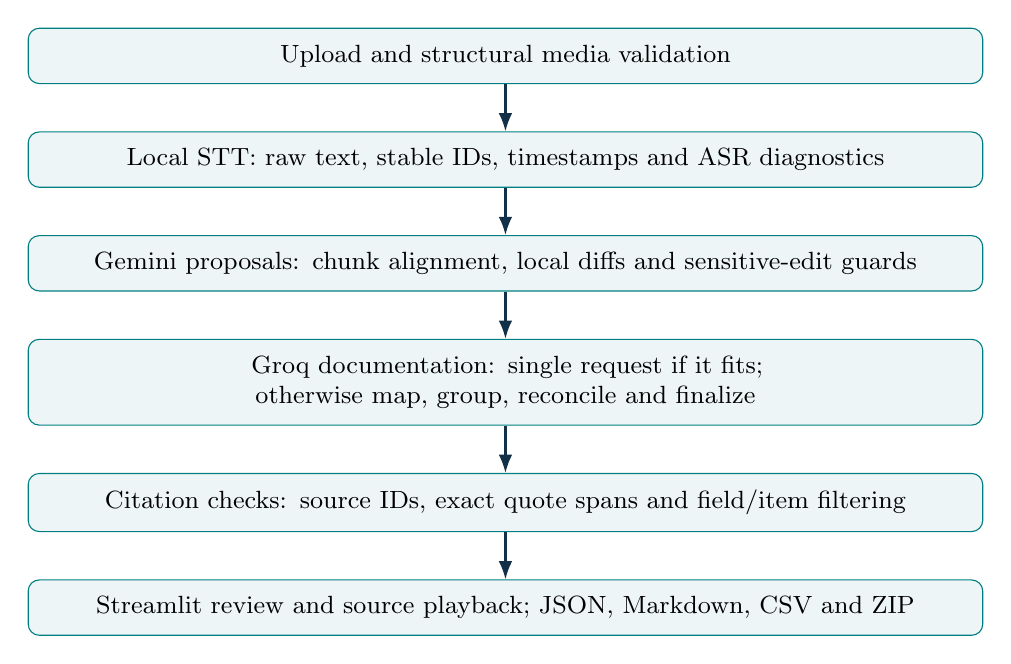
\begin{tikzpicture}[node distance=6mm,box/.style={draw=accent,fill=pale,rounded corners,text width=11.7cm,align=center,inner sep=6pt,font=\small},arr/.style={-{Latex},thick,draw=ink}]
\node[box](a){Upload and structural media validation};
\node[box,below=of a](b){Local STT: raw text, stable IDs, timestamps and ASR diagnostics};
\node[box,below=of b](c){Gemini proposals: chunk alignment, local diffs and sensitive-edit guards};
\node[box,below=of c](d){Groq documentation: single request if it fits; otherwise map, group, reconcile and finalize};
\node[box,below=of d](e){Citation checks: source IDs, exact quote spans and field/item filtering};
\node[box,below=of e](f){Streamlit review and source playback; JSON, Markdown, CSV and ZIP};
\foreach \x/\y in {a/b,b/c,c/d,d/e,e/f}\draw[arr](\x)--(\y);
\end{tikzpicture}
\end{center}

\subsection{Why Gemini was retained for refinement but replaced for minutes}
Initially both language roles used Gemini. Small preflight requests sometimes succeeded while documentation calls repeatedly failed with HTTP 503 and, in one sequence, HTTP 499. Importantly, small documentation probes also failed at times. This means the logs do not establish that transcript length alone caused the failures. Service availability, request latency and client cancellation were plausible contributors, not a proven root cause.

The implementation response was to change one role at a time. The successful refinement baseline stayed in place; Groq documentation was tested first on synthetic speech and then a short real transcript. This preserved a known stage and reduced the number of simultaneous changes. A synthetic probe returned the expected named-owner task and distinguished a rejected deployment proposal from an approved decision. That probe established a usable integration path, not broad model superiority.

Local Ollama models and larger speech models were considered. They were not promoted into the integrated profile because no comparative accuracy/runtime evidence had been collected. Installing an SDK alone would not establish an offline pipeline, and small local-model performance on long, ambiguous meetings remained unmeasured. The provider interface supports separation of concerns, but the current orchestration is explicitly Gemini-refinement/Groq-minutes; it is not automatic provider fallback.
\src{\code{config/default.yaml}; \code{tracemeet/llm/base.py}; \code{tracemeet/stages/minutes_workflow.py}}

\subsection{Other models considered for each role}
Model choice was driven by a usable CPU baseline, compatibility with structured contracts, observed access and recovery behavior, and the cost of changing a working stage. The following options are candidates for comparison, not experimentally ranked alternatives. Provider documentation establishes capabilities, not superiority on TraceMeet's recordings.

\small
\begin{longtable}{@{}>{\raggedright\arraybackslash}p{0.20\textwidth}>{\raggedright\arraybackslash}p{0.34\textwidth}>{\raggedright\arraybackslash}p{0.38\textwidth}@{}}
\toprule Role and option & Potential benefit & Trade-off and selection rationale\\\midrule\endhead
STT: selected Whisper \code{small.en} & Working English CPU/INT8 pipeline with local audio processing. & Selected as an accessible baseline. Its accuracy/runtime balance is not proven optimal.\\[5pt]
STT: Whisper \code{large-v3} or \code{distil-large-v3} & Alternative checkpoints supported by faster-whisper; Distil-Whisper offers an English-focused option~\cite{faster,distil}. & Larger-model deployment and device configuration require runtime/memory checks. No measured WER gain on this project justifies replacing the working baseline yet.\\[5pt]
Refinement: selected Gemini Flash-Lite & Already exercised with glossary context, chunked output and alignment validation. & Retaining it isolated the documentation-provider change. Cloud access and semantic correction quality still need monitoring.\\[5pt]
Refinement: Groq GPT-OSS 20B & A concrete alternative supported by the provider adapter and Groq's structured-output documentation~\cite{groq,gpt20}. & Could allow one provider account, while keeping a distinct minutes model. Harmful-edit rate, latency and quotas need measurement before adoption.\\[5pt]
Minutes: selected Groq GPT-OSS 120B & Produced usable structured records in the development probes and supports the implemented schema contract~\cite{groq}. & Selected on observed integration behavior, not parameter count as a quality score. Request allowance and pacing add latency.\\[5pt]
Minutes: Gemini Flash & Would retain a single cloud-provider setup and the earlier documentation implementation. & Repeated failures in development motivated the change. They do not establish that Gemini is generally less accurate or less reliable.\\[5pt]
Either LLM role: local instruction model through Ollama & Local serving supports schema-shaped responses~\cite{ollama}; locally stored models could reduce cloud dependence. & Ollama is a runtime, not a model. A specific checkpoint must be selected, downloaded and evaluated for memory, context, speed and accuracy. No tested local fallback is claimed.\\
\bottomrule
\end{longtable}
\normalsize

The selected combination is therefore a justified implementation baseline, not the outcome of a comprehensive model benchmark. Replacing either language model requires rechecking semantic behavior and not just whether JSON parses.

\subsection{Alternatives and trade-offs}
\begin{tabularx}{\textwidth}{@{}p{0.23\textwidth}YY@{}}\toprule
Design decision & Alternative considered & Trade-off accepted\\\midrule
CPU-capable local STT & Hosted STT or a larger local model & Avoids a speech API dependency; recognition quality and CPU runtime remain evaluation questions.\\
Segment-text refinement & Model-generated character-span edits & Simpler model contract; exact edit spans are computed locally after generation.\\
Read-only overlap & Rewriting overlapping target windows & One applied result per segment; context remains limited near larger discourse boundaries.\\
Strict citation presence & Fuzzy matching or global punctuation removal & Preserves exact provenance; valid paraphrases may be rejected and require regenerated evidence.\\
Whole-segment withholding & Apply only selected fragments of a risky proposal & Easier conservative auditing; useful edits can be withheld alongside risky ones.\\
Explicit mixed providers & Replace both language stages at once & Preserves a working refinement baseline; requires two keys and two provider error policies.\\
Budgeted long path & One unrestricted full-transcript request & Supports the configured allowance; adds latency and possible grouping/context errors.\\\bottomrule
\end{tabularx}

\section{Data contracts and provenance boundaries}
\subsection{Transcript identity}
A transcript comprises segments with a stable ID, start/end times and text. Segment IDs are unique, times are nonnegative, and each end must be no earlier than its start. Optional ASR fields include average log probability and no-speech probability. IDs are recording-local identifiers, not speaker identifiers or globally unique keys across meetings.

Let the raw transcript be $R=\{(i_k,t_k^s,t_k^e,x_k)\}_{k=1}^{n}$ and the refinement proposal be $P$. A valid refinement preserves the ordered identity sequence:
\[
[(i_k,t_k^s,t_k^e)]_{R}=[(i_k,t_k^s,t_k^e)]_{P}.
\]
Python restores timestamps from the original segments; the refiner is asked to produce revised text and IDs, not new temporal alignment.

\subsection{Meeting record}
The record contains a summary, organized minutes, decisions, action items and open questions. Decision states are decided, proposed, rejected and unresolved. Task states are confirmed and tentative. Evidence consists of a segment ID and quote. Owner and deadline are nullable, with separate evidence lists. The schema rejects an assigned owner without owner evidence and rejects owner evidence when the owner is absent; the same coupling applies to deadlines.

These contracts enforce shape and consistency between fields. They do not establish that the cited person is the speaker or that an owner was actually assigned. Missing values remain null in JSON and are displayed as ``Unspecified'' in readable views. The summary currently has no citation field and is explicitly described as an unverified overview.
\src{\code{tracemeet/schemas.py}}

\section{Audio validation and local transcription}
\subsection{Structural validation is not speech detection}
The media validator checks file existence, nonzero size, whether PyAV can open the container, and whether an audio track exists. It prefers the audio stream's duration when available, falls back to container duration, and rejects known durations below one second. Unknown duration is not silently interpreted as zero. Opening a container does not guarantee that every later frame can be decoded; decoding errors can still arise during transcription.

Silence and unreadable media are different conditions. The structural validator does not infer speech from signal amplitude. The transcriber enables VAD, and an empty decoded transcript produces a clear no-speech message. Audible noise, music or VAD acceptance still do not constitute proof of intelligible meeting speech.

\subsection{Transcription settings and progress}
Whisper provides the speech-recognition foundation~\cite{whisper}; faster-whisper implements inference using CTranslate2 and supports CPU INT8 execution~\cite{faster}. The local wrapper fixes English transcription, beam size five, VAD with a 500 ms minimum silence interval, and \code{condition_on_previous_text=False}. Optional names and terms are supplied as initial-prompt context and hotwords. Such hints can influence recognition and must not be treated as evidence that the terms were spoken.

faster-whisper returns a lazy segment iterator. The implementation consumes it inside the error boundary, removes blank output, assigns sequential IDs and converts diagnostics to validated fields. Tiny floating-point overshoot in no-speech probability is clamped within a narrow tolerance; genuinely invalid values are rejected. Progress follows decoded audio position and is set to completion after iteration, including recordings with trailing silence. It is not a reliable estimate of remaining wall-clock time.
\src{\code{tracemeet/audio/validate.py}; \code{tracemeet/stt/local_whisper.py}}

\section{Domain-aware refinement and correction logging}
\subsection{Read-only overlap and alignment}
The default refinement planner targets 25 segments per chunk and includes two neighbouring context segments on either side when available. Targets are disjoint; overlap is read-only context. This avoids competing rewrites for the same boundary segment. The 20,000-character request ceiling is enforced through chunk construction rather than rejecting every long meeting as a whole.

Responses must contain exactly the target IDs in input order. Missing, duplicated, unexpected or reordered IDs trigger alignment failure. One additional alignment-repair generation is permitted. The merged transcript is checked again, so local success does not bypass whole-transcript identity validation.

Each chunk checkpoint is identified by a hash of implementation version, provider, model, temperature, system prompt and payload. A cached response is schema-validated and alignment-checked before reuse. This saves quota on resume, although structural validation alone cannot detect every validly shaped manual content alteration to a checkpoint.

\subsection{Diffs are computed by Python}
The refiner does not generate trustworthy character offsets. Instead, \code{difflib.SequenceMatcher}~\cite{difflib} compares tokens that include whitespace, words and punctuation, with \code{autojunk=False}. Match-object positions map edits back to exact source and candidate slices:
\[
\text{original edit text}=x[\text{raw\_start}:\text{raw\_end}].
\]
The stored spans support highlighting and audit logs without asking an LLM to reproduce offsets. Metrics include changed segments, edit spans, whitespace-only spans, inserted/deleted tokens and replaced character totals. Non-whitespace token counts include punctuation; they are not equivalent to a linguistic word-error metric or the number of incorrect letters.

\subsection{Meaning-sensitive guards}
The guard compares ordered sequences of number expressions and sensitive vocabulary, including negation, commitments, dates/temporal markers and units. Currency/percentage symbols and counts of protected names are checked separately. A capitalization heuristic provides an additional cautious signal, not named-entity recognition.

Known contractions are normalized for comparison, including cannot/can not and can't/can not. The comparison retains repeated markers and order. Reducing negation checking to a boolean presence test was rejected because it could miss removal of one negation when another remains. Likewise, removing all punctuation before every check could hide meaningful number or currency changes.

If any sensitive flag is triggered, the entire segment retains raw wording. This conservative unit of acceptance avoids applying an apparently harmless fragment while a related risky edit is withheld. Accepted rewrites have raw ASR confidence fields cleared because those diagnostics describe the original recognized wording. Unchanged or withheld segments retain them.

For illustration only, a synthetic proposal that changes ``Morgan'' to ``Morgen'' should be withheld for name review. This example is not an excerpt from a meeting or a measured result. Acceptance means no configured heuristic fired; it is not proof the new wording is correct. The same capitalization safeguard can withhold valid technical corrections such as term capitalization or token joining. A meaningful evaluation must measure both harmful edits applied and beneficial edits unnecessarily blocked.
\src{\code{tracemeet/stages/refine.py}; \code{tracemeet/guards/diff.py}; \code{tracemeet/guards/sensitive.py}}

\section{Structured providers, errors and request budgets}
\subsection{Provider contracts}
Stages call \code{generate_structured(model, system, prompt, schema, temperature)} through a common interface. Gemini documents schema-based structured output~\cite{gemini}. The adapter passes a Pydantic-generated JSON schema through \code{response_json_schema}, rejects missing or incomplete candidates, and validates returned JSON locally. This followed an observed rejection of \code{additional_properties} in the earlier response-schema path.

Groq documents strict structured output for the GPT-OSS models~\cite{groq}. The adapter adapts a copied schema for strict output: defaults are removed, object properties become required, additional properties are disallowed, and nested schema structures are visited. It preserves actual property names such as \code{title}; accidentally deleting that field caused missing-title validation failures during reconciliation. Provider-constrained JSON still requires local validation of custom invariants.

\subsection{Input and completion planning}
For Groq, the estimator tokenizes system text, prompt and serialized schema using \code{o200k_harmony}. If their total is $N$, the planned request size is
\[
\widehat{T}=\lceil 1.10N\rceil+256+C,
\]
where $C$ is the completion reserve. Default values are budget 7,400, reserve 3,072, grouping reserve 2,048, and a 120-second HTTP timeout. These are configured engineering allowances, not measurements of an account's live quota or a guarantee of server token accounting.

A request is not sent when the estimate exceeds budget. The 463-segment example initially required an estimated 17,981 tokens including reserve, so it could not use the configured single-request path. A provider's model context capacity and an account's allowed request throughput are different constraints. The implementation chooses the long path rather than truncating transcript text.

\subsection{Bounded recovery rather than unlimited retries}
The Gemini adapter disables SDK retries and classifies 429 separately from transient 408/499/5xx codes. The router applies exponential backoff with jitter, reads structured retry hints, and stops on recognized daily-quota exhaustion or waits over 60 seconds. The default router limit is three total attempts. Refinement calls this default for each generation; the separate one-time alignment repair can introduce another bounded generation sequence. Historical minutes logs showing five attempts should not be mistaken for a universal current retry setting.

Groq generated-schema failures are distinguished from arbitrary HTTP 400 errors. Long stages permit bounded content/schema repair attempts. Network, timeout and general provider errors in the current Groq adapter stop with checkpoints retained; they are not all automatically retried by the Gemini-oriented router. This distinction makes operational limitations explicit.
\src{\code{tracemeet/llm/gemini.py}; \code{tracemeet/llm/groq_provider.py}; \code{tracemeet/llm/router.py}}

\section{Long-meeting documentation}
\subsection{Why independent chunk summaries are insufficient}
A task proposed early can be cancelled later, and an owner or deadline can change after a topic break. Simply concatenating independent chunk summaries would conceal these relationships. TraceMeet instead uses provisional extraction, meeting-wide grouping, source-grounded reconciliation and accounted finalization. This reduces the risk; it does not guarantee global semantic consistency when extraction or grouping is wrong.

\subsection{Map: observations with source identity}
The map stage extracts topics, proposals, agreements, tasks, rejections, amendments, cancellations and open questions. Each observation must cite at least one target segment; allowed neighbouring context can supply additional support. Unknown or duplicated citation IDs are rejected. In the current map design, the model returns source IDs and Python retrieves source text, avoiding model-generated quotation copying in this stage.

An early contract asked the model to return all processed target IDs. It sometimes returned only IDs relevant to observations, causing coverage failures even with valid observations. The revised contract records supplied targets in Python and retains source IDs on observations. This removed redundant model bookkeeping, not traceability. The correct claim is that every input segment was supplied exactly once as a target, not that every fact was understood or extracted.

\subsection{Group: assign observations across the meeting}
Grouping considers observations from the entire meeting. A dynamic schema provides one required assignment field per observation; Python checks complete, unique assignment and materializes discussion groups. Compact representation reduces schema/prompt overhead while preserving observations. The grouping operation remains model-dependent: two related statements can still be placed in different groups.

The current implementation does not recursively solve every possible grouping-budget overflow. A meeting with too many observations, or a single very large discussion group, can still require further design work or a verified larger allowance. ``Long-meeting support'' therefore denotes budget-aware decomposition and recoverability, not unlimited duration.

\subsection{Reconcile: return to source speech}
Each group is reconciled using its observations and relevant source segments with neighbouring context. The model produces draft minutes, decisions, tasks and questions. Python materializes evidence from allowed IDs and applies schema and anchoring checks. Later changes are intended to supersede earlier statements when the supplied source supports that interpretation. The group jobs are budget-checked before reconciliation calls; an oversized group stops rather than silently dropping source.

\subsection{Finalization: no silent disappearance of existing candidates}
Each provisional task, decision and question receives a stable candidate ID. Review responses must account for every candidate exactly once with retain, revise, merge or remove. Non-removal entries reference outputs; removed candidates carry reasons but no output index. Validation rejects missing/duplicated candidate coverage, cross-kind merging, unaccounted outputs, and retain actions that change substantive fields. Review evidence must anchor each consumed candidate to its original primary source.

This replaces the earlier failure mode in which a shorter output could silently lose tasks. It does not prove that a removal reason is correct, and it cannot recover a fact never extracted into any candidate. Whole discussion groups are preserved in review batching, while related source citations and nearby context are supplied for interpretation.

\subsection{Overview: plan for output as well as input}
An overview request once fit its input budget but exhausted completion tokens before producing required \code{omitted_topics}. The updated planner constrains both estimated input and topic workload. Its heuristic capacity is
\[
K=\max\left(1,\left\lfloor\frac{C-768}{128}\right\rfloor\right),
\]
which gives 18 source topics at a 3,072-token reserve. It also reserves 192 tokens of request headroom for retry feedback. Whole groups remain intact; groups that cannot fit cause a clear failure. This is a planning heuristic, not a completion guarantee.

Every source topic must appear in condensed-topic references or an explicit omission with a reason. Python restores supporting evidence. Multiple batch summaries are joined into the final overview; there is no additional unlimited whole-meeting synthesis call. This preserves budget control but can produce repetition or weaker cross-batch coherence.
\src{\code{tracemeet/stages/minutes_map.py}; \code{minutes_group.py}; \code{minutes_reconcile.py}; \code{minutes_finalize.py}}

\section{Evidence verification and source playback}
A citation is accepted only if its segment exists and its quote occurs as an exact contiguous substring without cutting through a word. The search continues after an invalid partial-word occurrence so a later valid occurrence can be found. Empty or punctuation-only evidence is rejected. A short quote that omits trailing punctuation can already match as a substring; global punctuation deletion or fuzzy similarity is not needed for that case.

The verifier records character bounds and the segment's start/end times. Those timestamps refer to the whole segment, not word-level alignment of the quoted substring. Clicking evidence selects the corresponding audio/video region in the interface; the user can then listen to context.

A minutes topic, decision or question is dropped when any required citation fails. A task with invalid primary evidence is dropped. If primary evidence passes but owner or deadline evidence fails, that field is cleared to null and its evidence list removed. The candidate is not mutated, and the checked output is validated again. Reports preserve original candidate paths, exclusions and limitations.

\textbf{Why exact presence is insufficient.} In a synthetic example, the quote ``We should not deploy on Friday'' contains the exact substring ``deploy on Friday''. A claim that deployment was approved can therefore carry a valid substring but an invalid interpretation. Similar problems arise with quotations of other speakers, rejected proposals and unresolved pronouns. TraceMeet checks citation presence and exposes context; it does not claim a complete semantic verifier.
\src{\code{tracemeet/guards/evidence.py}; \code{tracemeet/ui/results.py}}

\section{Orchestration, persistence and reproducibility}
\subsection{Stage fingerprints and downstream invalidation}
The pipeline stores media, raw/proposed/refined transcripts, meeting candidates, citation reports and stage state in a run folder. A stage fingerprint hashes relevant inputs and source-file dependencies with a stage/version identifier. Saved stage artifacts must also match their recorded file hashes before reuse. Changing an upstream input invalidates that stage and downstream completion entries, while matching completed work can be reused.

This mechanism allows a documentation failure to preserve transcription and refinement. It also detects artifact edits that would otherwise be mistaken for current results. Dependency lists are explicit: a newly introduced dependency must be added to the appropriate fingerprint inputs. Installed package versions are not automatically covered by these source-file hashes; the dependency snapshot is a separate reproducibility control.

\subsection{Disk state, locking and legacy runs}
Pipeline state includes status, current stage, error, attempt history, stage durations, settings and artifact provenance. Writes use a temporary file followed by replacement. A per-run exclusive lock prevents two pipeline sessions from writing the same run. A crashed process can leave a stale lock; recovery should first establish that no writer remains. This is not a cross-process account-wide quota scheduler.

Legacy imports verify available model/settings/hash links and label their provenance. They do not pretend to know the historical code version. Compatibility checks accept known byte-hash and normalized-text-hash representations where appropriate. This addressed a Windows-era mismatch in which the raw file hash matched metadata but a text-read/re-encode comparison differed.

A reported Windows \code{WinError 5} occurred during replacement of \code{run_state.json}. Resume later completed. The precise locking/permission cause was not established, and the current atomic-replace helper is not a demonstrated universal fix for Windows file contention.

\subsection{Three meanings of reproducibility}
\begin{description}
\item[Environment reproducibility:] dependency files and the lock snapshot describe setup; a fresh-machine installation still needs verification.
\item[Artifact reproducibility:] matching saved outputs can be reopened with hashes, schemas and source links checked.
\item[Inference repeatability:] regenerating a cloud output may differ, even with identical settings. Temperature zero is not a proof of bitwise determinism.
\end{description}
The system supports auditable artifact reuse. It should not be described as fully deterministic or fully evaluated end-to-end reproducibility before clean-clone and independent evaluation gates are completed.
\src{\code{tracemeet/pipeline.py}; \code{requirements.lock.txt}}

\section{Interactive review and export design}
\subsection{Features that make the pipeline inspectable}
The Streamlit interface provides recording upload, contextual terms, protected names, model-role display, processing status and saved-run recovery. Preview is skipped above 50 MiB; source playback can be opted into for larger recordings. It is possible to download transcript artifacts even when later documentation fails.

The correction inspector shows raw wording, the model proposal and the wording actually passed to documentation. Exact offsets support highlights, and HTML-escaped text is used when rendering marked spans. Withheld proposals are labeled. Interactive accept/reject/custom correction was requested as a future improvement but is not implemented in this version.

Meeting results separate confirmed tasks from tentative actions and display decision status. Users can inspect owner/deadline evidence, the original candidate, citation exclusions and finalization review reasons. Those reasons remain model-generated explanations, not independent semantic proof.

Run storage retains stable identifiers. Display labels combine date, the first available minutes topic and original filename, with an optional custom title. They are not generated by a new summary-to-title model call. Presentation metadata is separate from inference inputs so renaming a meeting need not regenerate it.

\subsection{Single-record export contract}
The export builder validates raw/refined identity, runs citation checks and renders all formats from the same checked record. The ZIP includes meeting JSON, Markdown, task CSV, raw and refined transcript JSON, evidence report, notes and a SHA-256 manifest. Audio and the guard correction report are not included by this bundle builder; correction artifacts remain available in the run/UI.

CSV contains evidence fields, uses a UTF-8 BOM for common Windows spreadsheet workflows and prefixes formula-like cells with an apostrophe. JSON preserves the underlying values. Consequently consistency means equivalent record content under documented presentation transformations, not byte-identical text in every format. The UI displays readable results directly; corporate users are not required to inspect JSON to understand the meeting.
\src{\code{tracemeet/ui/results.py}; \code{tracemeet/ui/run_labels.py}; \code{tracemeet/export/bundle.py}; \code{csv_export.py}}

\section{Development failures and resulting design changes}
\small
\begin{longtable}{@{}>{\raggedright\arraybackslash}p{0.23\textwidth}>{\raggedright\arraybackslash}p{0.34\textwidth}>{\raggedright\arraybackslash}p{0.35\textwidth}@{}}
\toprule Observed problem & Engineering response & What the evidence supports\\\midrule\endhead
Gemini HTTP 404 and intermittent 503/499 & Preflight access checks, detailed errors, explicit transient classes; minutes role moved to Groq. & Access and availability varied. A single transcript-size root cause was not established.\\[5pt]
Gemini schema field rejection & Use JSON-schema request field and retain local Pydantic validation. & Request/schema compatibility was repaired for observed calls.\\[5pt]
Long refinement hit a character ceiling & Bounded target chunks, read-only overlap, alignment checks and checkpoints. & Long input can be decomposed without changing segment identity.\\[5pt]
Dangerous or ambiguous term changes & Whole-segment sensitive guards and visible proposals. & Some risky edits were withheld; semantic safety is not guaranteed.\\[5pt]
Groq long input exceeded budget & Token-aware routing and staged documentation. & No silent input truncation was needed for the logged long run.\\[5pt]
Quote crossed two source segments & Prompt correction for short path; ID-based quote retrieval in long stages. & The verifier detected the mismatch; source IDs remained central.\\[5pt]
Map output omitted processing IDs & Python records supplied coverage, model returns observation evidence. & Complete input accounting replaces unreliable self-reported coverage.\\[5pt]
Grouping lost assignments & Required assignment per observation and Python uniqueness checks. & Structural grouping coverage is checked, not semantic group quality.\\[5pt]
Missing minutes title & Preserve actual schema properties during adaptation. & Diagnosed local validation errors became actionable.\\[5pt]
Finalization silently reduced candidates & Explicit dispositions and exact candidate/output accounting. & Existing candidates cannot disappear without a recorded disposition.\\[5pt]
Overview output was truncated & Input/output-aware batching and explicit topic omissions. & Capacity planning improved; output length remains model-dependent.\\[5pt]
Internet interruption during map & Resume validated completed chunk checkpoints. & Logs showed earlier chunks reused without repeated inference.\\[5pt]
Streamlit reload/model identity mismatch & Reconstruct validated Pydantic objects from plain data. & Validation is retained across class-identity changes.\\[5pt]
UI integration regressed old expectations & Update orchestration mocks and integrity-aware fixtures; restore proposal/partial-result features. & Recorded regression suite subsequently passed.\\
\bottomrule
\end{longtable}
\normalsize

\section{Validation evidence and limits}
\subsection{Evidence basis and observed results}
The results below are taken from recorded development logs and manual workflow checks. They are not averages from a controlled evaluation. The developer reported 246 tests passing in 6.33 seconds at the supplied source revision. This test run was not repeated during report preparation. The two included development clips are each 300 seconds, 16 kHz, mono and originate from the same longer recording; they do not form an independent held-out set. Only aggregate operational results are reported here. No third-party meeting transcript or participant names are reproduced.

\begin{tabularx}{\textwidth}{@{}p{0.25\textwidth}YY@{}}\toprule
Check & Observed result & Interpretation\\\midrule
Regression suite & Developer log: 246 passed in 6.33 s at the supplied source revision. & Regression evidence; not a fresh-clone test or an accuracy score.\\
Short Groq sample & 21 segments; 3.1 s on one logged request; 19 exact matches after prompt revision. & Demonstrated short-path integration on that sample.\\
Long documentation & 463 segments, 72 provisional observations and 13 groups in logs. & Demonstrated staged processing; not a ground-truth completeness score.\\
Accounted finalization & 19 minutes, 1 decision, 12 tasks, 13 questions; 375 exact citation matches. & Recorded run outcome; semantic accuracy still required inspection.\\
UI smoke tests & Manual checks confirmed withheld wording, timestamp playback and ZIP opening; two five-minute workflows completed. & Manual end-to-end behavior on development clips.\\
Archive media & Both WAV headers: 300 s, 16 kHz, mono. & Independently inspected file properties, not content quality.\\\bottomrule
\end{tabularx}

The long-record counts changed materially across revisions, including an earlier output with five tasks and a later output with twelve. That difference motivated explicit disposition accounting. More tasks are not automatically better; a reviewer must determine whether the additional items are genuinely actionable and whether removed items were duplicates, tentative offers or unsupported assignments.

\subsection{Packaged five-minute examples}
The developer identified the two export bundles as belonging to the corresponding sample WAVs. Offline inspection checked every exported manifest hash, raw/refined segment identity, CSV/JSON task consistency and citation spans against the supplied refined transcripts. The original exports were preserved byte for byte.

\begin{tabularx}{\textwidth}{@{}Yrr@{}}\toprule
Artifact property & Sample 1 & Sample 2\\\midrule
Duration (seconds) & 300 & 300\\
Raw transcript segments & 91 & 68\\
Minutes topics & 15 & 5\\
Decisions & 1 & 0\\
Action items & 1 & 1\\
Open questions & 0 & 1\\
Exact citation occurrences & 53 & 19\\
Invalid citations & 0 & 0\\
Manifest hash mismatches & 0 & 0\\\bottomrule
\end{tabularx}

These counts describe the exported records, not extraction precision or recall. Citation occurrences include repeated use of the same evidence. The exports contain no source-audio hash, so the audio-to-bundle pairing is developer-supplied rather than independently established by a media fingerprint. Redistribution permission for the source recording must be confirmed before publishing the sample package. Neither clip is an independent held-out evaluation.

\subsection{Latency and quota trade-offs}
The integrated long path shares a 61-second post-request gap between its main and grouping providers. Stage-local waits account for time already elapsed. If $m$ sequential uncached requests share this pacing, the pacing contribution alone is approximately $(m-1)61$ seconds, plus model/network time and any repair calls. This is a conservative configured policy, not an intrinsic model latency or a universal provider requirement.

This policy can make long meetings take many minutes and is a usability limitation. Checkpoint reuse reduces repeated cost after failure. A future quota-aware scheduler could use verified account limits and response headers, but blindly shortening waits or adding parallel calls would risk new rate-limit failures. No measured cost-per-meeting or complete long-run runtime is claimed from partial logs.

\subsection{Required accuracy evaluation}
A defensible evaluation needs human reference transcripts and annotated decisions/tasks, ideally with two-pass adjudication of ambiguous speech. The current two clips share a source meeting and cannot be counted as independent held-out meetings. A separate recording should remain untouched by prompt tuning.

For transcription, report $\mathrm{WER}=(S+D+I)/N$ under a declared normalization policy, for both raw and guarded refined text. Also score domain terminology, because aggregate WER can hide changes to high-value names or technical terms. Review each proposed correction as beneficial, harmful or neutral, and report both applied harmful edits and beneficial edits withheld.

For decisions and tasks, define matching criteria before scoring. Report precision $TP/(TP+FP)$ and recall $TP/(TP+FN)$, with explicit zero-denominator handling. Evaluate status, owner and deadline correctness separately; do not allow an approximately correct description to conceal an invented assignee. Track unsupported owner/deadline counts, citation validity, extraction omissions, latency, API failures and resume behavior.

The raw-versus-refined ablation should hold documentation prompts/model/settings fixed and vary only the transcript supplied. Both outputs need the same annotation standard. All these accuracy metrics are pending at this report revision; no placeholder numeric scores are presented.

\section{Security, privacy and remaining limitations}
Recordings are transcribed locally, but transcript text and contextual terms are sent to cloud language providers. Users must decide whether their recordings are appropriate for those services. Keys are environment-based, errors redact configured keys, and private run data should stay out of source control. Local files are not an encrypted enterprise datastore.

Prompts describe transcript content as data rather than instructions. This is a useful prompt-level boundary, not a proven defense against all prompt injection. Guards and exact citations are also incomplete semantic controls. A malicious or mistaken statement can be quoted exactly; source presence does not certify truth.

Without reliable speaker identification, a first-person statement such as the synthetic example ``I will send the report'' does not identify a named owner. The intended policy is to leave that owner unspecified unless explicit source evidence resolves the identity. Citation checks alone cannot guarantee that the model obeys this policy.

Important current limitations are lack of diarization, incomplete owner/commitment verification, an uncited summary, heuristic sensitive-word coverage, possible grouping mistakes, and finalization views that do not reread every source segment. Request and output budgets bound supported workloads. Model access, free-tier quotas, throughput and stochastic behavior can change. The default workflow processes English only. Per-run locks do not coordinate all jobs using one API key, and atomic replacement can still encounter platform errors.

The highest-value future work is a labeled evaluation set, audited human correction approval, stronger status/assignment checks, evidence-bearing summaries and measured quota-aware scheduling. A tested local provider and speech-model comparisons remain separate future experiments rather than claims about the delivered application.

\section{Reproduction and submission procedure}
\begin{enumerate}
\item Clone the submitted repository revision and create a Python 3.11 virtual environment.
\item Install the supplied lock snapshot and run pip's dependency check. Record installation errors instead of silently changing versions.
\item Configure Gemini and Groq keys locally. Run offline configuration checks, then small live probes with explicit quota awareness.
\item Start Streamlit, upload a new short English recording and inspect every stage through citation checks and exports.
\item Trigger a controlled later-stage failure and confirm that matching earlier stages are reused on resume. Keep model inputs/configuration unchanged for this check.
\item Test missing keys and invalid media. Open the ZIP and compare its record with the UI.
\item Preserve a shareable recording with its actual generated outputs, exact configuration, source commit and usage permissions. Record the demo from a real run.
\end{enumerate}

The repository contains source, prompts, setup files, an MIT license and two development samples. Private run artifacts are not part of the source release. A paired sample-output package has been prepared and checked offline. Public distribution still requires confirmation of source-recording permission. The final submission still needs the demonstration video, clean-clone evidence and any completed accuracy measurements. The full technical report complements the short technical description; it does not replace those validation deliverables.

\section*{Acknowledgments}
\addcontentsline{toc}{section}{Acknowledgments}
The author acknowledges the maintainers and contributors of Whisper, faster-whisper, CTranslate2, PyAV, Pydantic, Streamlit and the Python ecosystem, together with the Gemini and Groq API documentation and services used during development. Their software and documentation enabled the implementation described here. These acknowledgments do not imply endorsement of TraceMeet or its results.

\appendix
\section{Source map}
\begin{tabularx}{\textwidth}{@{}lY@{}}\toprule
Source area & Responsibility\\\midrule
\code{app.py}, \code{pages/} & Upload, processing entry and saved-run access\\
\code{tracemeet/pipeline.py} & State, dependencies, invalidation and recovery\\
\code{tracemeet/stt/}, \code{audio/} & Local STT and structural validation\\
\code{tracemeet/llm/} & Provider requests, budgets and error boundaries\\
\code{tracemeet/stages/} & Refinement and short/long documentation\\
\code{tracemeet/guards/} & Diff spans, sensitive edits and citation presence\\
\code{tracemeet/ui/}, \code{export/} & Inspection, playback, labels and output formats\\
\code{tests/}, \code{eval/guard_stats.py} & Regression tests and guard statistics\\\bottomrule
\end{tabularx}

\textbf{Repository:} \url{https://github.com/adityaomsah/TraceMeet}

For reproduction, retain the submitted Git revision together with configuration, dependency versions and generated run metadata. Full revision identifiers and archive checksums belong in release metadata rather than the report narrative. The source references above identify the modules implementing each stage.

\section{Operational commands}
From the repository root in Windows PowerShell:
\begin{lstlisting}
py -3.11 -m venv .venv
.\.venv\Scripts\python.exe -m pip install -r requirements.lock.txt
.\.venv\Scripts\python.exe -m pip check
.\.venv\Scripts\python.exe -m scripts.preflight_pipeline --offline
.\.venv\Scripts\python.exe -m scripts.preflight_pipeline
.\.venv\Scripts\python.exe -m pytest tests -q
.\.venv\Scripts\python.exe -m streamlit run app.py
\end{lstlisting}
The live preflight consumes quota; the offline preflight checks configuration and key presence without model inference. Do not include real keys in the report, screenshots or Git history.

\section{Interpretation checklist for reviewers}
\begin{itemize}
\item A completed stage means its implemented checks passed, not that every semantic claim is correct.
\item A citation match confirms a quote exists; listen to the surrounding segment before trusting status or attribution.
\item A guarded transcript contains only accepted proposals, with withheld segments preserved raw.
\item A candidate disposition prevents silent loss of an existing candidate; it does not prove extraction completeness.
\item Reusing a checkpoint reproduces a saved artifact, not a fresh model response.
\item Recorded sample results and test counts are not substitutes for an annotated held-out evaluation.
\end{itemize}

\clearpage
\addcontentsline{toc}{section}{References}
\begin{thebibliography}{9}
\bibitem{whisper} A. Radford, J. W. Kim, T. Xu, G. Brockman, C. McLeavey, and I. Sutskever. \emph{Robust Speech Recognition via Large-Scale Weak Supervision}. arXiv:2212.04356, 2022. \url{https://arxiv.org/abs/2212.04356}.
\bibitem{faster} SYSTRAN and contributors. \emph{faster-whisper: Faster Whisper transcription with CTranslate2}. Repository documentation. \url{https://github.com/SYSTRAN/faster-whisper}.
\bibitem{distil} Distil-Whisper project. \emph{distil-large-v3 model card}. \url{https://huggingface.co/distil-whisper/distil-large-v3}.
\bibitem{gemini} Google AI for Developers. \emph{Structured outputs, Gemini API}. Official documentation. \url{https://ai.google.dev/gemini-api/docs/structured-output}.
\bibitem{groq} Groq. \emph{Structured Outputs}. Official documentation. \url{https://console.groq.com/docs/structured-outputs}.
\bibitem{gpt20} Groq. \emph{OpenAI GPT-OSS 20B}. Model documentation. \url{https://console.groq.com/docs/model/openai/gpt-oss-20b}.
\bibitem{ollama} Ollama. \emph{Structured Outputs}. Official documentation. \url{https://docs.ollama.com/capabilities/structured-outputs}.
\bibitem{difflib} Python Software Foundation. \emph{difflib: Helpers for computing deltas}. Python documentation. \url{https://docs.python.org/3/library/difflib.html}.
\end{thebibliography}

\end{document}
